\section{The limiting conditional distribution}
\label{sec:qsd}

It is often the case in stochastic processes, as it is here for $p<\tfrac12$, that
fixation to a particular state is inevitable. In certain cases, though, long before
absorption the process settles into a distribution that no longer changes with time ---
one that describes the population conditional on its not yet having been absorbed. This
phenomenon is called quasi-stationarity, and the distribution it converges to is the
quasi-stationary, or Yaglom, limit \cite{Yaglom1947,Athreya1972}. This section
establishes it for the binary Galton--Watson process by computing the limiting
conditional mean and variance.

\subsection{Late-time survival probability}
\label{sec:lateS}

Everything follows from the behaviour of $S_n$. Take $p<\tfrac12$, so that death of an
individual is more probable than its reproduction. Then $S_n\to0$, and as it does so
the quadratic term in
\begin{equation*}
S_{n+1} = 2pS_n - pS_n^2
\end{equation*}
becomes negligible beside the linear one. The recursion is therefore increasingly well
approximated by
\begin{equation}
\label{attenuated}
S_{n+1} \approx 2p\,S_n,
\end{equation}
and so at late times
\begin{equation}
\label{lateS}
S_n \sim A(p)\,(2p)^n \qquad (n\to\infty),
\qquad
A(p) = \lim_{n\to\infty}\frac{S_n}{(2p)^n}.
\end{equation}
The constant $A(p)$ absorbs the cumulative effect of the quadratic term over the early
generations, before the linear regime takes hold: it is what remains of the lingering
conditions on $S_n$ accumulated before attenuation to \cref{attenuated}. The limit exists
and is finite and strictly positive for $p\in[0,\tfrac12)$; a proof via an infinite
product is given in \cref{sec:product}, and \cref{sec:Abounds} locates it in
$(0,\tfrac12]$.

\begin{remark}
The relation \cref{lateS} is an asymptotic equivalence, not an identity. The limit of
$S_n$ itself is $0$ for $p<\tfrac12$, and one must not write
$\lim_n S_n = A(p)(2p)^n$: the right-hand side still depends on $n$. What is being
asserted is that the ratio $S_n/(2p)^n$ converges.
\end{remark}

\subsection{Mean}
\label{sec:condmean}

Decompose the expected population size into the contributions from surviving and extinct
realisations:
\begin{equation*}
\mean{\zz_n}
= \pr{\zz_n = 0}\,\cancelto{0}{\mean{\zz_n\mid \zz_n = 0}}
+ \pr{\zz_n > 0}\,\mean{\zz_n \mid \zz_n > 0}.
\end{equation*}
The first term vanishes identically, so with $\pr{\zz_n>0}=S_n$,
\begin{equation}
\label{eq:condmeandef}
\mean{\zz_n \mid \zz_n > 0} = \frac{\mean{\zz_n}}{S_n} = \frac{(2p)^n}{S_n},
\end{equation}
using $\mean{\zz_n}=(2p)^n$ from \cref{eq:meanZn}. We know what $(2p)^n$ does; the
content is all in $S_n$, and \cref{lateS} supplies it:
\begin{equation}
\label{eq:qsmean}
\mean{\zz_n \mid \zz_n > 0} \;\xrightarrow[n\to\infty]{}\; \frac{(2p)^n}{A(p)(2p)^n} = \frac{1}{A(p)}.
\end{equation}
The geometric factors cancel exactly. At late times the surviving population has a
constant expected size, and that size is the reciprocal of $A(p)$. For this reason
$1/A(p)$ is referred to below as the quasi-stationary mean.

\Cref{fig:condmean} shows the convergence. It also shows the difficulty that
\cref{sec:Ap} will have to confront: the closer $p$ is to $\tfrac12$, the higher the
plateau and the longer the process takes to reach it.

\begin{figure}[ht]
\centering
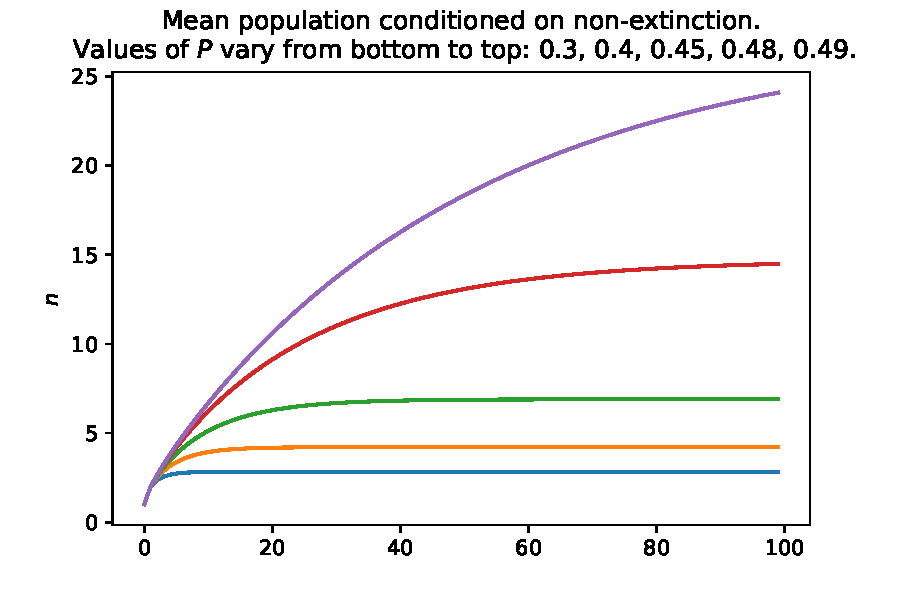
\includegraphics[width=0.78\textwidth]{figures/IMG_ch3/conditionalMean.pdf}
\caption{The conditional mean $(2p)^n/S_n$ plotted against generation number $n$,
with $S_n$ computed by iterating \cref{SnIter}. From bottom to top,
$p = 0.3,\,0.4,\,0.45,\,0.48,\,0.49$. Each curve approaches the constant $1/A(p)$;
the values are $2.825$, $4.208$, $6.893$, $14.703$ and $27.476$ respectively,
computed as in \cref{sec:practical}. The lowest three have essentially converged by
$n=100$, but the $p=0.49$ curve has reached only $24.1$ of its limiting $27.5$ ---
an early sign of the near-critical slowdown discussed in \cref{sec:practical}.
(The vertical axis is mislabelled $n$ in the original plotting script; it is the
conditional mean.)}
\label{fig:condmean}
\end{figure}

\subsection{Variance}
\label{sec:variance}

The mean is not the whole of quasi-stationarity. To show that the conditional
distribution settles down we need at least the second moment, and computing it is a
worthwhile exercise in its own right.

\subsubsection{The second moment $\mean{\zz_n^2}$}

For a random variable $\xx$ the moment generating function is $\mean{\ee^{t\xx}}$, which
can be written in terms of the \pgf{} as $\phi(\ee^t)$. For the binary offspring law
\cref{eq:pgfbinary},
\begin{equation}
\label{mgf1}
M_1(t) = \phi_1(\ee^t) = p\,\ee^{2t} + (1-p),
\end{equation}
the subscript $1$ indicating relevance to generation $n=1$. Moments follow from
\begin{equation}
\label{mgf2}
\mean{\zz_n^r} = \frac{\dd^r}{\dd t^r}M_n(t)\bigg|_{t=0}.
\end{equation}
For the second moment of $\zz_1$, differentiating \cref{mgf1} twice and evaluating at
$t=0$ gives
\begin{equation*}
\frac{\dd^2}{\dd t^2}M_1(t)\bigg|_{t=0} = 4p\ee^{2t}\big|_{t=0} = 4p.
\end{equation*}
That is only the first generation. To reach generation $n$ we must dig a little deeper.
Recall that the $n$-step \pgf{} is the $n$-fold composition
\begin{equation*}
\phi_n(z) = \underset{n\ \text{times}}{\underbrace{\phi_1\lrb{\phi_1\lrb{\dots\phi_1\lrb{z}}}}},
\end{equation*}
so that
\begin{equation*}
M_n(t) = \phi_1\lrbq{\phi_1\lrbq{\dots\phi_1\lrbq{\ee^t}}}.
\end{equation*}
Differentiating once by the chain rule,
\begin{equation}
\label{dmgf1}
M_n'(t) = \phi_1'\lrbq{\phi_{n-1}\lrbq{\ee^t}}\cdot\phi_1'\lrbq{\phi_{n-2}\lrbq{\ee^t}}\cdots\phi_1'\lrbq{\phi_{1}\lrbq{\ee^t}}\cdot\phi_1'\lrbq{\ee^t}\cdot\ee^t .
\end{equation}
Now
\begin{equation*}
\phi_1'\lrbq{\phi_k\lrbq{\ee^t}}
= \frac{\dd}{\dd\,\phi_k\lrbq{\ee^t}}\Bigl(p\bigl[\phi_k\lrbq{\ee^t}\bigr]^2 + (1-p)\Bigr)
= 2p\,\phi_k\lrbq{\ee^t},
\end{equation*}
and $\phi_1'\lrbq{\ee^t} = 2p\ee^t$, so \cref{dmgf1} collapses to
\begin{equation*}
M_n'(t) = (2p)\phi_{n-1}\lrbq{\ee^t}\cdot(2p)\phi_{n-2}\lrbq{\ee^t}\cdots(2p)\phi_{1}\lrbq{\ee^t}\cdot(2p)\ee^{2t},
\end{equation*}
that is,
\begin{equation}
\label{dmgf2}
M_n'(t) = (2p)^n\cdot M_{n-1}(t)\cdot M_{n-2}(t)\cdots M_1(t)\cdot\ee^{2t}.
\end{equation}
Before differentiating again, note that every factor here equals $1$ at $t=0$:
$M_k(0)=1$ for all $k$, and $\ee^{0}=1$. This is what makes the second derivative
tractable. Differentiating the product \cref{dmgf2} gives a sum of terms, each identical
to \cref{dmgf2} except that one factor has been differentiated:
\begin{align*}
M_n''(t) = (2p)^n\bigg[\,&M_{n-1}'(t)\cdot M_{n-2}(t)\cdots M_1(t)\cdot\ee^{2t}\\
+ &M_{n-1}(t)\cdot M_{n-2}'(t)\cdots M_1(t)\cdot\ee^{2t}\\
&\hspace{60pt}\vdots\\
+ &M_{n-1}(t)\cdot M_{n-2}(t)\cdots M_1'(t)\cdot\ee^{2t}\\
+ &M_{n-1}(t)\cdot M_{n-2}(t)\cdots M_1(t)\cdot 2\ee^{2t}\,\bigg].
\end{align*}
At $t=0$ all the undifferentiated factors become $1$, leaving
\begin{equation*}
M_n''(0) = (2p)^n\lrbs{M_{n-1}'(0) + M_{n-2}'(0) + \cdots + M_1'(0) + 2}.
\end{equation*}
But $M_k'(0)$ is just the mean population at generation $k$, namely $(2p)^k$, so
\begin{equation*}
M_n''(0) = (2p)^n\lrbs{(2p)^{n-1} + (2p)^{n-2} + \cdots + (2p) + 2}
= (2p)^n\lrbs{\sum_{i=0}^{n-1}(2p)^i + 1}.
\end{equation*}
Summing the finite geometric series,
\begin{equation*}
\mean{\zz_n^2} = M_n''(0) = (2p)^n\lrbs{\frac{1-(2p)^n}{1-2p} + 1},
\end{equation*}
and rearranging,
\begin{equation}
\label{secondMoment}
\mean{\zz_n^2} = (2p)^n\lrb{1 + \frac{1}{1-2p}} - (2p)^{2n}\lrb{\frac{1}{1-2p}}.
\end{equation}
The minus sign is required: at $n=1$ the expression must return $\mean{\zz_1^2}=4p$,
which it does.

\subsubsection{Late-time variance}

From $\text{Var}(\zz_n) = \mean{\zz_n^2}-\mean{\zz_n}^2$ and \cref{secondMoment},
\begin{equation*}
\text{Var}(\zz_n) = (2p)^n\lrb{1 + \frac{1}{1-2p}} - (2p)^{2n}\lrb{\frac{1}{1-2p}} - (2p)^{2n}.
\end{equation*}
For $2p<1$ the terms in $(2p)^{2n}$ are negligible beside $(2p)^n$ at large $n$, so
\begin{equation*}
\text{Var}(\zz_n) \to (2p)^n\lrb{1 + \frac{1}{1-2p}}.
\end{equation*}
It is tempting to read stationarity of the conditional variance straight off this, but
that would be too quick: the conditional variance is not the unconditional one divided
by anything simple. Start instead from the conditional moments. Using \cref{lateS},
\begin{align*}
\mean{\zz_n^2\mid \zz_n\neq0} &= \frac{\mean{\zz_n^2}}{S_n}
\;\xrightarrow{n\to\infty}\;
\frac{(2p)^n\lrb{1+\frac{1}{1-2p}}}{A(p)(2p)^n} = \frac{1}{A(p)}\lrb{1+\frac{1}{1-2p}},\\[4pt]
\mean{\zz_n\mid \zz_n\neq0} &= \frac{\mean{\zz_n}}{S_n}
\;\xrightarrow{n\to\infty}\;
\frac{(2p)^n}{A(p)(2p)^n} = \frac{1}{A(p)}.
\end{align*}
Both limits are finite, so the conditional variance does indeed tend to a constant:
\begin{equation}
\label{eq:condvar}
\text{Var}(\zz_n\mid \zz_n\neq0) \;\longrightarrow\; \frac{1}{A(p)}\lrb{1+\frac{1}{1-2p}} - \frac{1}{A(p)^2}.
\end{equation}
The first two moments of the conditional population therefore both stabilise, and the
same argument extended to higher moments gives the full quasi-stationary distribution.
Note that \cref{eq:condvar}, like \cref{eq:qsmean}, is expressed entirely in terms of
$p$ and the single unknown constant $A(p)$. Everything now turns on that constant.

\subsection{A continuum view of the survival recursion}
\label{sec:riccati}

Before turning to $A(p)$ proper it is useful to record a continuum approximation that
recurs later. Writing $r = 1-2p$ for the distance from criticality, the recursion
\cref{SnIter} rearranges to
\begin{equation}
\label{eq:Sdiff}
S_{n+1}-S_n = -r S_n - p S_n^2 .
\end{equation}
For large $n$ the unit increment is small on the scale over which $S$ varies, and the
left-hand side is well approximated by a derivative, giving the Riccati equation
\begin{equation}
\label{eq:riccati}
\frac{\dd S}{\dd n} = -r S - p S^2 .
\end{equation}
Substituting $u = 1/S$ linearises it, $u' = ru + p$, with solution
$u(n) = K\ee^{rn} - p/r$ and hence
\begin{equation}
\label{eq:riccatisol}
S(n) = \frac{r}{K r\,\ee^{rn} - p},
\end{equation}
$K$ a constant fixed by the initial condition. Setting $r=0$ recovers the critical
scaling $S\sim2/n$ of \cref{twoovrn_sn}; keeping $r>0$ recovers the geometric decay
$S\sim A(p)(2p)^n$ of \cref{lateS}, since $(2p)^n = \ee^{\,n\ln(1-r)}$ agrees with
$\ee^{-rn}$ to leading order in $r$. The constant $K$ is exactly the object that the
continuum approximation cannot supply, because it is determined by the early generations
where the approximation is invalid --- which is another way of saying that it is $A(p)$,
and that no argument of this kind will produce it. \Cref{sec:asymptotic} shows how much
can nevertheless be extracted near criticality.

\FloatBarrier
